%!TEX program = xelatex
\documentclass[cn,hazy,blue,10pt,normal]{elegantnote}
\title{商业决策平台的智能数据管理系统分析报告}

\author{卢羿舟}
\institute{统计与数据科学系}

% \version{2.50}
% \date{\zhdate{2022/12/31}}

\usepackage{array}
\usepackage{natbib}
\usepackage{algorithm}
\usepackage{algpseudocode}
\usepackage{dirtree}

\usepackage{listings} % 引入 listings 宏包
\usepackage{xcolor}   % 用于定义颜色

% --- listings 的 Python 样式定义 (可选,可根据喜好调整) ---
\lstdefinestyle{mystyle}{
    language=Python,
    backgroundcolor=\color{lightgray!20}, % 背景颜色
    commentstyle=\color{green!70!black},    % 注释颜色
    keywordstyle=\color{blue},            % 关键词颜色
    numberstyle=\tiny\color{gray},        % 行号样式
    stringstyle=\color{purple},           % 字符串颜色
    basicstyle=\ttfamily\footnotesize,    % 基本字体样式
    breakatwhitespace=false,              % 只在空格处断行
    breaklines=true,                      % 自动断行
    captionpos=t,                         % 标题位置 (b=底部, t=顶部)
    keepspaces=true,                      % 保留空格
    numbers=left,                         % 行号位置 (left, right, none)
    numbersep=5pt,                        % 行号与代码的距离
    showspaces=false,                     % 不显示空格符号
    showstringspaces=false,               % 不显示字符串中的空格符号
    showtabs=false,                       % 不显示制表符
    tabsize=2,                            % 制表符宽度
    frame=lines,                         % 添加边框 (single, lines, none, ...)
    rulecolor=\color{black},              % 边框颜色
    title=\lstname                        % 显示文件名作为标题 (如果从文件读入)
}
\lstset{style=mystyle} % 应用自定义样式

\begin{document}

\maketitle
\tableofcontents


\newpage
\setcounter{page}{1}

\section{项目背景}
在当今快速发展和竞争激烈的商业环境中,企业对于精准、高效的决策能力的需求日益增长。为了应对这一挑战,构建一个强大的商业决策平台显得尤为重要。本项目的核心目标是打造该平台底层的智能数据管理模块,旨在对关键业务数据进行高效处理和分析,从而为上层决策提供坚实的数据支撑。

本项目需要为一家新兴数据驱动商业决策平台设计底层数据处理模块。该平台存储的主要数据包括:
\begin{enumerate}
    \item 营销任务:储存任务的名称,紧急度,影响力
    \item 表示营销任务间前置依赖的有向图
    \item 表示客户关系的加权有向图
    \item 商品数据:包括商品名称、价格、热度
\end{enumerate}
其中所有数据类型均为数字或英文。基于这些数据,项目需要实现以下分析模块:
\begin{enumerate}
    \item 营销任务优先调度模块
    \item 客户网络与影响力传播分析模块
    \item 商品数据检索模块
\end{enumerate}
具体而言,\textbf{营销任务优先调度模块}维护一个存储所有营销任务的结构。
该结构需要有基础的插入、删除、更改营销任务的功能,并支持执行优先级最高的任务、查看优先级最高的前$k$个任务等高级操作,其中,一个任务的优先级定义为其紧急度和影响力的乘积。同时,需要考虑营销任务之间的前置依赖关系。在第\ref{sec: marketingtask}节详细讨论了该模块的设计与实现。
\textbf{客户网络与影响力传播分析模块}基于存储客户之间关系的加权有向图进行分析。需要评估每一位客
户的重要性,并寻找每一位客户能影响到的所有其他客户,同时,当客户之间的影响路径过长或者影响力过小的时候,忽略两客户之间的影响。在第\ref{sec: customer}节详细讨论了该模块的设计与实现。
\textbf{商品数据检索模块}需要实现一个外存高效的数据结构来实现商品数据的增删改查,同时实现支持通过商品名进行前缀搜索。在第\ref{sec: goods}节详细讨论了该模块的设计与实现。

除此之外,本报告在第\ref{sec: src}节介绍了项目源代码结构,在第\ref{sec: improvement}节讨论了由于时间关系其他因素导致该项目不完善的地方。对于附录,本报告在附录\ref{sec: demo}中演示了运行\texttt{app.py}的方法以及运行结果,在附录\ref{sec: unittest}中展示了运行单元测试的方法以及项目每一个部分的单元测试代码,其中包含了具体的测试用例和测试方法。最后在附录\ref{sec: llm}对项目开发过程中使用的LLM代码工具进行了详细的说明。

\newpage
\section{源代码文件树说明\footnote{这里省略了Python运行时产生的缓存文件。}}
\label{sec: src}

\dirtree{%
.1 /.
.2 docs/.
.3 Project Guidelines.pdf\DTcomment{该项目的要求说明}.
.2 src/.
.3 \_\_init\_\_.py.
.3 data\_structure/.
.4 \_\_init\_\_.py.
.4 b\_plus\_tree.py\DTcomment{B+树}.
.4 customer\_graph.py\DTcomment{有向赋权图}.
.4 dependency\_graph.py\DTcomment{有向无环图}.
.4 updatable\_max\_heap.py\DTcomment{支持快速查找的优先队列}.
.4 trie.py\DTcomment{Trie树}.
.3 model/.
.4 \_\_init\_\_.py.
.4 marketing\_task.py\DTcomment{MarketingTask类}.
.4 product.py\DTcomment{Product类}.
.3 module/.
.4 \_\_init\_\_.py.
.4 commodity\_retrieval.py\DTcomment{商品数据检索模块}.
.4 customer\_network\_analysis.py\DTcomment{客户网络与影响力传播分析模块}.
.4 marketing\_task\_schedule.py\DTcomment{营销任务优先调度模块}.
.3 utils.py\DTcomment{一些可视化函数}.
.2 tests/.
.3 \_\_init\_\_.py.
.3 test\_b\_plus\_tree.py\DTcomment{B+树测试代码}.
.3 test\_customer\_graph.py\DTcomment{有向赋权图测试代码}.
.3 test\_dependency\_graph.py\DTcomment{有向无环图测试代码}.
.3 test\_dfs\_influence.py\DTcomment{影响力传播算法测试代码}.
.3 test\_marketing.py\DTcomment{营销任务调度测试代码}.
.3 test\_pagerank.py\DTcomment{PageRank算法测试代码}.
.3 test\_product.py\DTcomment{Product类测试代码}.
.3 text\_trie.py\DTcomment{Trie树测试代码}.
.3 test\_updatable\_max\_heap.py\DTcomment{支持快速查找的优先队列测试代码}.
.3 test\_weighted\_degree\_centrality.py\DTcomment{度中心性算法测试代码}.
.2 app.py\DTcomment{系统入口,Demo程序}.
}

% \texttt{docs}文件夹包括对该项目的要求说明,\texttt{src}中为本项目的主要实现代码,其中\texttt{data\_stricture}目录里为所有额外用到的数据结构实现,而\texttt{module}文件夹中包含了三个模块的具体实现。最后\texttt{tests}文件夹包含所有的测试用例。

\newpage
\section{设计思路与功能分析}
该部分包括了对项目需要实现的三个模块的设计思路、实现方法、重要算法的时间与空间复杂度分析等内容。
\label{sec: design}

\subsection{营销任务优先调度模块}
\label{sec: marketingtask}

\subsubsection{模块功能拆解与分析}
该模块需要实现一个储存所有营销任务的数据结构,该数据结构支持对营销数据的增、删、改,同时需要根据营销任务的具体性质,自动计算其优先级。优先级的计算是明确的,定义为$\text{紧急度}\times\text{影响力}$。随后利用计算得到的优先级,考虑任务之间的相互依赖后优先执行优先级最高的任务,同时能展示任务优先级最高的$k$个任务\footnote{由于项目要求并未说明当考虑任务相互依赖关系后,在展示任务优先级最高的$k$个任务时是否考虑任务前置依赖,由于这两种需求的实现方式类似,所以本项目在实现时仅实现了一种可能,展示的是考虑任务前置依赖下的$k$个优先级最高的任务,只有不存在前置依赖的任务才会被展示。对于不考虑任务优先级的示任务优先级最高的$k$个任务,实现原理与方法类似,故不再过多陈述。}。

该模块最重要的任务是根据任务的优先级进行排列,执行优先度最高的任务与查看优先级最高的$k$个任务的要求最为符合堆的特点,所以该模块需要维护的一个核心数据结构为最大堆,堆顶始终储存优先级最高的营销任务。对于查看优先级最高的$k$个任务,由于并未提前指定$k$,所以无法直接使用一个控制大小为$k$的堆。对于这个功能的实现,有两个方案
\begin{enumerate}
    \item 每次调用该功能时,将最大堆连续弹出$k$个节点,储存后再插入恢复;
    \item 每次调用该功能时,复制一份最大堆,然后进行破坏性弹出。
\end{enumerate}
考虑在实际生产环境中,可能存在大量营销任务,复制一份最大堆需要的空间复杂度过高,因此在本模块的实现中最终选择了第一个方案。

为了考虑任务之间的前置依赖关系,我们需要实现一个有向图,图中的每个节点均为一个营销任务,边的指向代表了任务之间的依赖关系,具体而言,我们规定
\begin{align*}
    \text{前置任务} \longrightarrow \text{后置任务}
\end{align*}
为有向图的存储规则。由于任务之间存在依赖关系,为了更好的管理任务状态,我们考虑为任务附加一个属性$\mathtt{\_status}$,用来表示任务当前的状态。我们将任务的状态分成三类:$\mathtt{Pending}$,$\mathtt{Ready}$和$\mathtt{Complete}$,分别代表三种状态:该任务存在前置依赖,该任务不存在前置依赖与该任务已完成。通过维护任务依赖关系有向图来区分$\mathtt{Pending}$和$\mathtt{Ready}$的任务,同时考虑仅将状态为$\mathtt{Ready}$的任务加入可以执行的最大堆。这样就实现了同时考虑任务优先级和前置依赖关系的营销任务规划\footnote{由于时间原因,暂时实现了该较为简单的算法,在第\ref{sec: improvement}节中还讨论了另一个更加完善的版本。}。

最后,考虑任务列表的增、删、改。注意到这三个操作都有可能直接或者间接的影响任务之间的依赖关系和优先级,其中修改任务可能会修改任务的紧急度和影响力,进而影响任务优先级,而增和删可能破坏原有的依赖结构,让原本处于$\mathtt{Ready}$状态的任务重新回到$\mathtt{Pending}$,所以为了让最大堆能够高效地适应这些变化,我们需要让这个最大堆拥有可以直接查找的特性。考虑到这种增、删、改的操作可能是频繁的,在堆中额外维护一个查找字典是一个好的选择,尽管这样做会增加需要的存储空间,但是相比于每次查找都遍历堆来说,这种额外开销是可以接受的。因此,为了让任务能够存储在字典中,我们为定义了$\mathtt{\_task\_id}$,这个属性是任务被创建时候定义的,且在营销任务整个生命周期都不能改变,相比之下任务的名称是可以被改变的。生成$\mathtt{\_task\_id}$的规则为“时间戳-UUID”。考虑合并时间戳与UUID来作为ID是因为我们既希望每一个任务的ID独一无二,又希望它是有序的,好管理的。我们可以直接在所有的数据结构中均使用ID来进行统一管理。

\subsubsection{功能实现}
为了实现上述的功能,在该模块中,总共实现了四个类,分别为
\begin{itemize}
    \item $\mathtt{MarketingTask}$
    \item $\mathtt{TaskManager}$
    \item $\mathtt{UpdatableMaxHeap}$
    \item $\mathtt{TaskDependencyGraph}$
\end{itemize}
其中$\mathtt{MarketingTask}$表示每个任务对象,$\mathtt{TaskManager}$为储存营销任务并进行规划的类,这个类中主要维护以下两个数据结构:$\mathtt{UpdatableMaxHeap}$和$\mathtt{TaskDependencyGraph}$。他们分别用来实现根据优先级进行排列的优先队列和表示任务之间依赖关系的有向图。下面具体讲解每一个类的实现方式。

\textbf{$\mathtt{MarketingTask}$类}

在实现这个类之前,首先定义了三个常量
\begin{itemize}
    \item $\mathtt{TASK\_STATUS\_PENDING}$
    \item $\mathtt{TASK\_STATUS\_READY}$
    \item $\mathtt{TASK\_STATUS\_COMPLETED}$
\end{itemize}
分别表示不同的任务状态。考虑到这个类会被反复、大量初始化,为了节约内存,使用了$\mathtt{\_\_slots\_\_}$命令。在这个类中总共有六个属性,分别为
\begin{itemize}
    \item $\mathtt{\_task\_id}$
    \item $\mathtt{\_name}$
    \item $\mathtt{\_status}$
    \item $\mathtt{urgency}$
    \item $\mathtt{influence}$
    \item $\mathtt{\_priority}$
\end{itemize}
通过$\mathtt{@property}$和$\mathtt{setter}$来控制对这些私有变量的访问和修改。其中$\mathtt{\_priority}$并不直接初始化,而是在$\mathtt{urgency}$和$\mathtt{influence}$初始化和改动时自动计算并修改。这一设计让这个类本身变得相对更加安全,拒绝了可能会导致错误的改动,也实现了调用的方便,不再需要重新写get函数来实现对私有变量的访问。同时,$\mathtt{MarketingTask}$类还包含两个私有方法
\begin{itemize}
    \item $\mathtt{\_update\_details()}$\footnote{注意,由于美观性以及空间因素,在本分析报告中所有出现的函数都默认不填写参数名和参数类型,详细的参数说明可以参考源代码注释。}:更新任务的紧急程度或者影响力,并更新优先级,如果某个参数为None,则不更新该属性,如果更新成功,则返回True,如果没有更新,则返回False
    \item $\mathtt{\_set\_status()}$:设置任务的状态
\end{itemize}
前者负责更新该任务的可修改描述,如紧急度、影响力、名称等,后者负责设置任务的状态。$\mathtt{MarketingTask}$类不直接暴露这些方法,是因为我们只希望在$\mathtt{TaskManager}$内部修改$\mathtt{MarketingTask}$的状态。

\textbf{$\mathtt{TaskDependencyGraph}$类}

为了实现高效查找节点和依赖关系,在$\mathtt{TaskDependencyGraph}$类我们使用了两个字典,分别储正向依赖关系以及反向依赖关系,以及一个集合用于存储任务ID。其中正向依赖关系指的是从某个任务节点指向其他后续任务的映射,而反向依赖关系指的是某个任务节点被哪些任务前置影响的映射。这个类中包含了常规的图应有的方法,包括
\begin{itemize}
    \item $\mathtt{add\_task()}$:向图中添加一个任务节点
    \item $\mathtt{remove\_task()}$:从图中移除一个任务节点及其所有相关依赖, 并返回这个节点id
    \item $\mathtt{add\_dependency()}$:添加依赖关系:$\text{prerequisite\_id}$ -> $\text{dependent\_id}$,在添加前会进行环路检测
    \item $\mathtt{remove\_dependency()}$:移除依赖关系:$\text{prerequisite\_id}$ -> $\text{dependent\_id}$
    \item $\mathtt{get\_dependents()}$:获取直接依赖于$\text{task\_id}$的任务集合
    \item $\mathtt{get\_prerequisites()}$:获取$\text{task\_id}$的前置任务集合
    \item $\mathtt{has\_task()}$:检查任务是否存在于图中
    \item $\mathtt{get\_all\_tasks()}$:返回图中所有任务的列表
\end{itemize}
分别用于节点的增加、删除,边的增加、删除,获取正向依赖关系,获取反向依赖关系,判断节点是否在图中以及获取图中所有的任务列表。值得注意的是,在这个模块背景中,依赖关系应该是一个无环图,否则环路上的任务将永远也无法满足前置条件。因此在添加边的时候,需要检测添加这条边后会不会导致环路出现。这个检测的原理即通过深度优先搜索寻找是否存在一条待添加边的反向通路,倘若存在,则不允许添加这条边,否则会导致图中出现环。这个深度优先搜索是通过一个私有方法$\mathtt{\_has\_path()}$实现的。这个方法通过列表模拟栈来实现了一个迭代式的深度优先搜索,可以根据搜索结果来确定是否可以在图中添加一条前置关系。另一个值得注意的是当使用$\mathtt{remove\_task()}$这个方法时,除了该任务,同时会删除所有和这个任务相关的边,包括前置和后置边。

\textbf{$\mathtt{UpdatableMaxHeap}$类}

这个数据结构本质是一个利用以列表实现的最小堆模拟的最大堆(存入负优先级),同时为了支持高效的删除和查找操作,这个类额外维护了一个位置映射字典,它用于将堆中存放的任务ID映射到该任务在列表中的索引,以此来实现对堆的高效查找和删除。这个类存在一系列最小堆的私有方法,用于实现查找父节点、左右子节点和节点交换、上浮和下沉。值得注意的是,由于我们额外添加了一个位置映射字典,所以在常规最小堆的$\mathtt{\_swap()}$的基础上,额外添加一步对位置映射的修改。由于上浮和下沉操作完全依赖交换操作,所以仅需要改动这里一处即可。

对于这个数据结构的公共接口,和常规最小堆的公共接口也没有太大的区别,只是需要在插入和删除的时候,增添一步对位置映射的更新即可。除此之外额外添加了一个$\mathtt{update\_priority()}$方法,该方法搜索给定的任务ID,然后更新该任务在堆中的优先级,然后重新上浮或者下沉该任务节点。下面展示这个数据结构的公共接口列表。
\begin{itemize}
    \item $\mathtt{insert()}$:向堆中插入一个新任务,如果任务已存在,则更新优先级
    \item $\mathtt{peek\_max()}$:查看堆顶元素, 不移除
    \item $\mathtt{extract\_max()}$:移除并返回堆顶元素
    \item $\mathtt{is\_empty()}$:检查堆是否为空
    \item $\mathtt{update\_priority()}$:更新堆中已存在任务的优先级
    \item $\mathtt{delete()}$:从堆中删除指定任务ID的元素
    \item $\mathtt{get\_heap\_size()}$:返回堆中元素的数量
\end{itemize}


\textbf{$\mathtt{TaskManager}$类}

这个类是该模块的核心类,用于实现所有营销任务优先调度模块需要实现的功能。它维护了多个数据结构:
\begin{itemize}
    \item $\mathtt{\_tasks}$:字典,任务ID到任务对象的映射
    \item $\mathtt{\_task\_graph}$:$\mathtt{TaskDependencyGraph}$类,储存任务之间的依赖关系
    \item $\mathtt{\_ready\_queue}$:$\mathtt{UpdatableMaxHeap}$类,储存所有状态为Ready的任务的优先队列
    \item $\mathtt{\_in\_degree}$:字典,状态为Pending的任务ID到其前置依赖数量的映射
\end{itemize}
这个类通过入度字典监控所有的任务状态,当任务状态发生变化时(如出现任务和任务关系的增删改),按照相应要求更新Ready队列,以保证所有处于Ready队列中的任务均为Ready状态。同时提供了一个执行任务的方法,即从Ready队列中选择优先度最高的任务取出,并更新任务状态为完成,随后考虑该任务的后继任务,同步更新入度字典和Ready队列。此外,创建新任务的时候,会用$\mathtt{\_generate\_task\_id()}$为任务赋予一个独一无二的任务ID,组成为“时间戳-UUID”。下面展示这个类的公共接口
\begin{itemize}
    \item $\mathtt{add\_task()}$:往任务管理器中添加一个任务
    \item $\mathtt{add\_dependency()}$:添加一个任务间的依赖关系,如果添加的依赖会导致后继任务不再ready,则需要将其从ready队列中移除
    \item $\mathtt{remove\_dependency()}$:移除一个已经存在的依赖关系,如果移除成功且导致后继任务的状态变为ready,则更新ready队列
    \item $\mathtt{mark\_task\_as\_completed()}$:将指定任务标记为已完成,同时更新其后续任务的入度字典
    \item $\mathtt{execute\_next\_highest\_priority\_task()}$:从ready队列中提取优先级最高的任务,并执行
    \item $\mathtt{get\_top\_k\_ready\_tasks()}$:查看当前ready队列中的优先级最高的k个任务
    \item $\mathtt{update\_task\_info()}$:更新现有的任务信息,如果更新的信息会导致优先级的变化,那么如果这个任务处于ready状态,会改变其在ready队列中的位置
    \item $\mathtt{delete\_task()}$:从系统中彻底删除一个任务及其所有相关依赖,包括
        1. 任务列表中的任务
        2. 前置依赖图中的节点和依赖的边
        3. ready队列中的任务(如果存在)
        4. 更新该任务的后置任务的入度字典,并考虑是否将失去前置条件的任务加入ready队列
        5. 把该任务从入度字典中删除
\end{itemize}

这个类实现时需要注意的细节为,需要在所有可能改变依赖关系和优先级顺序的操作下监控任务状态,其余需要注意的细节都已经被抽象到之前定义的数据结构中完成了。

\subsubsection{时间和空间复杂度分析}
在这一节中,我们将分析该模块使用到的数据结构以及重要算法的时间和空间复杂度。要分析的数据结构包括
\begin{itemize}
    \item $\mathtt{TaskDependencyGraph}$类
    \item $\mathtt{UpdatableMaxHeap}$类
\end{itemize}
由于$\mathtt{TaskManager}$类的操作均为依赖以上两个数据结构接口的逻辑判断,所以在此不做更多的分析。

首先对$\mathtt{TaskDependencyGraph}$类进行分析。考察数据结构的整体空间复杂度,有
\begin{itemize}
    \item $\mathtt{self.nodes}$,空间复杂度为$O(V)$
    \item $\mathtt{self.adj}$,空间复杂度为$O(V+E)$
    \item $\mathtt{self.rev\_adj}$,空间复杂度为$O(V+E)$
\end{itemize}
所以数据结构整体的空间复杂度为$O(V+E)$。

下面考虑不同方法的时间和空间复杂度。

\begin{itemize}
    \item $\mathtt{add\_task()}$:向字典中添加一个新元素,时间和空间复杂度均为$O(1)$,其中时间复杂度为摊销时间复杂度\footnote{在接下来,我们使用$O^*(\cdot)$来标记摊销时间复杂度。}。
    \item $\mathtt{remove\_task()}$:由于需要遍历所有节点,且涉及创建列表副本,所以时间复杂度为$O^*(V)$。而由于创建了前置和后置依赖的副本,所以空间复杂度为$O(V)$。
    \item $\mathtt{\_has\_path()}$:注意到这是一个标准的DFS,所以时间复杂度为$O^*(V+E)$,而空间复杂度为$O^(V)$。
    \item $\mathtt{add\_dependency()}$:该方法的主要时间和空间复杂度来自于$\mathtt{\_has\_path()}$,所以这个方法的时间复杂度为$O^*(V+E)$,空间复杂度为$O^(V)$。
    \item $\mathtt{remove\_dependency()}$:这个方法主要为字典查找和删除,所以时间复杂度和空间复杂度分别为$O^*(1)$和$O(1)$。
    \item $\mathtt{get\_dependents()}$:尽管查找步骤的时间复杂度为$O(1)$,但是由于胃了防止可变对象被外部修改,返回的是结果的副本,因此时间复杂度为$O^*(V)$,空间复杂度为$O(V)$。
    \item $\mathtt{get\_prerequisites()}$:同上,时间复杂度为$O^*(V)$,空间复杂度为$O(V)$。
    \item $\mathtt{has\_task()}$:时间复杂度为$O^*(1)$,空间复杂度为$O(1)$。
    \item $\mathtt{get\_all\_tasks()}$:时间复杂度为$O^*(V)$,空间复杂度为$O(V)$。
\end{itemize}

以上分析的结果总结可以查看表\ref{tab: task_graph complexity}。下面我们继续对$\mathtt{UpdatableMaxHeap}$类的分析。显然,该数据结构本身的空间复杂度为$O(N)$。

\begin{itemize}
    \item $\mathtt{insert()}$:无论是插入还是更新,都涉及堆的上浮与下沉操作,加上位置映射字典的更新,时间复杂度为$O^*(\log N)$,空间复杂度为$O(1)$。
    \item $\mathtt{peek\_max()}$:查看堆顶,时间和空间复杂度均为$O(1)$。
    \item $\mathtt{extract\_max()}$:从堆顶取出节点,涉及位置映射字典的更新与下沉操作,时间复杂度为$O^*(\log N)$,空间复杂度为$O(1)$。
    \item $\mathtt{is\_empty()}$:时间和空间复杂度均为$O(1)$。
    \item $\mathtt{update\_priority()}$:涉及查找与更新堆,并更新位置映射字典,所以时间复杂度为$O^*(\log N)$,空间复杂度为$O(1)$。
    \item $\mathtt{delete()}$:类似地,同样以上浮和下沉操作为主,时间复杂度为$O^*(\log N)$,空间复杂度为$O(1)$。
    \item $\mathtt{get\_heap\_size()}$:时间和空间复杂度均为$O(1)$。
\end{itemize}

对$\mathtt{UpdatableMaxHeap}$类的分析总结可以查看表\ref{tab: heap_complexity}。


\begin{table}[t]
    \centering
    \caption{TaskDependencyGraph方法复杂度分析}
    \label{tab: task_graph complexity}
    \begin{tabular}{lcc}
    \toprule
    方法  & 时间复杂度 & 空间复杂度 \\
    \midrule
    \texttt{add\_task()} & $O^*(1)$ & $O(1)$ \\
    \texttt{remove\_task()} & $O^*(V)$ & $O(V)$ \\
    \texttt{\_has\_path()} & $O^*(E + V)$ & $O(V)$ \\
    \texttt{add\_dependency()} & $O^*(E + V)$ & $O(V)$ \\
    \texttt{remove\_dependency()} & $O^*(1)$ & $O(1)$ \\
    \texttt{get\_dependents()} & $O^*(V)$ & $O(V)$ \\
    \texttt{get\_prerequisites()} & $O^*(V)$ & $O(V)$ \\
    \texttt{has\_task()} & $O^*(1)$ & $O(1)$ \\
    \texttt{get\_all\_tasks()} & $O^*(V)$ & $O(V)$ \\
    \bottomrule
    \end{tabular}
\end{table}



% \begin{table}[t]
%     \centering
%     \caption{UpdatableMaxHeap方法复杂度分析}
%     \label{tab: heap_complexity}
%     \begin{tabular}{lcc}
%     \toprule
%     方法  & 时间复杂度  & 空间复杂度  \\
%     \midrule
%     \texttt{insert()} & $O^*(\log N)$ & $O(1)$ \\
%     \texttt{peek\_max()} & $O(1)$ & $O(1)$ \\
%     \texttt{extract\_max()} & $O^*(\log N)$ & $O(1)$ \\
%     \texttt{is\_empty()} & $O(1)$ & $O(1)$ \\
%     \texttt{update\_priority()} & $O^*(\log N)$ & $O(1)$ \\
%     \texttt{delete()} & $O^*(\log N)$ & $O(1)$ \\
%     \texttt{get\_heap\_size()} & $O(1)$ & $O(1)$ \\
%     \bottomrule
%     \end{tabular}
% \end{table}


\subsection{客户网络与影响力传播分析模块}
\label{sec: customer}


\subsubsection{模块功能拆解与分析}
这个模块需要实现对客户关系网络的分析。首先我们定义所有客户与相互的影响关系被储存在一个有向图(这里的图可以有环)中,每个节点均表示一个客户。他们之间的影响关系如下
\begin{align*}
    \text{客户}A \overset{0.8}{\longrightarrow} \text{客户}B
\end{align*}
代表客户A可以直接影响客户B,而边权代表客户A对客户B的影响程度,这个数值的取值范围为了分析方便被限制在了$(0,1]$,数值越大代表影响程度越深,从而依靠这种关系来构建整个有向图。在这个模块中总共有两个分析任务:
\begin{enumerate}
    \item 客户重要性评价
    \item 寻找每一位客户所能影响到的所有客户
\end{enumerate}
这两个任务都是图数据结构中十分经典的任务。对于客户重要性评价,本质上是对有向图中的节点重要性进行评价。这样的评价指标有许多。在这个项目中,我们选择了两个比较经典的算法:加权度中心性和PageRank。下面简要介绍。

\begin{table}[t]
    \centering
    \caption{UpdatableMaxHeap方法复杂度分析}
    \label{tab: heap_complexity}
    \begin{tabular}{lcc}
    \toprule
    方法  & 时间复杂度  & 空间复杂度  \\
    \midrule
    \texttt{insert()} & $O^*(\log N)$ & $O(1)$ \\
    \texttt{peek\_max()} & $O(1)$ & $O(1)$ \\
    \texttt{extract\_max()} & $O^*(\log N)$ & $O(1)$ \\
    \texttt{is\_empty()} & $O(1)$ & $O(1)$ \\
    \texttt{update\_priority()} & $O^*(\log N)$ & $O(1)$ \\
    \texttt{delete()} & $O^*(\log N)$ & $O(1)$ \\
    \texttt{get\_heap\_size()} & $O(1)$ & $O(1)$ \\
    \bottomrule
    \end{tabular}
\end{table}

\begin{algorithm}[t]
\caption{适用于有向赋权图的PageRank 算法}
\label{alg:weighted_pagerank}
\begin{algorithmic}[1]
\Require 有向赋权图 $G=(V, E, W)$;阻尼因子 $d$;最大迭代次数 $N_{max}$;收敛阈值 $\epsilon$。
\Ensure 各节点 $u \in V$ 的 PageRank 得分 $PR[u]$。

\State 若 $V$ 为空, 则返回空结果。
\State \textbf{预处理:} 计算图中各节点的入链信息 $InMap[u]$ (包含源节点 $v$ 及权重 $W_{vu}$) 及加权出度 $W_{out}[v]$。
\State \textbf{初始化:} 对所有节点 $u \in V$, $PR[u] \leftarrow 1 / |V|$。

\For{$iteration = 1$ \textbf{to} $N_{max}$}
    \State $PR_{old} \leftarrow PR$
    \State $S_{dangling} \leftarrow \sum_{v \in V \text{ s.t. } W_{out}[v]=0} PR_{old}[v]$ \Comment{计算悬挂节点的PageRank总和}
    
    \For{每个节点 $u \in V$}
        \State $P_{links} \leftarrow 0$
        \If{$InMap[u]$ 非空}
            \For{每个 $(v, W_{vu}) \in InMap[u]$}
                \If{$W_{out}[v] > 0$}
                    \State $P_{links} \leftarrow P_{links} + \frac{PR_{old}[v] \cdot W_{vu}}{W_{out}[v]}$
                \EndIf
            \EndFor
        \EndIf
        \State $PR[u] \leftarrow \frac{1-d}{|V|} + d \cdot P_{links} + d \cdot \frac{S_{dangling}}{|V|}$
    \EndFor
    
    \If{$\sum_{u \in V} |PR[u] - PR_{old}[u]| < \epsilon$}
        \State \textbf{break} \Comment{已收敛}
    \EndIf
\EndFor

\State \Return $PR$
\end{algorithmic}
\end{algorithm}

要衡量一个图中节点的重要性,一个很直观的方法就是看他的入边和出边有多少。这类似于评价一个交通枢纽的重要程度,它能够连接起越多的路,一般而言就越重要。这个评价指标就被称为加权度中心性(\textbf{W}eighted \textbf{D}egree \textbf{C}entrality),加权度中心性越高,代表节点的重要性越高。在有向赋权图中,这个指标进一步变为加权入度中心性(WIDC)和加权出度中心性(WODC),这是为了区分不同边的性质和不同的边权,具体计算方式如下
\begin{align*}
    WIDC(o) = \sum_{u \in in(o)} w(u, o),\quad WODC(o) = \sum_{u\in out(o)} w(o, u),
\end{align*}
其中$in(o)$和$out(o)$分别代表节点$o$的所有入射节点和出射节点。

然而,度中心性存在一个很显然的问题:它没办法衡量相距超过$1$的点之间的影响。在我们的例子中,客户A如果能通过客户B而对C有影响,那么客户A的重要程度也应该能传导到对客户C的重要程度的评价上,而度中心性显然无法衡量这一影响。因此为了给管理者提供更加全面的决策参考,我们引入了PageRank算法~\citep{Page1999ThePC}来衡量节点重要性。PageRank最开始被用于评价网页重要性,其核心思想基于这样一种直观的理念:一个网页的重要性取决于指向它的其他网页的数量和质量。简单来说,PageRank 算法模拟了一个在互联网上随机冲浪的用户。用户从一个随机的网页开始,然后不断地点击页面上的链接。一个网页被访问的概率越高,那么这个网页就被认为越重要。具体来说,PageRank算法将互联网看作一个有向图,其中网页是节点,网页之间的链接是边。每个网页的PageRank值(PR值)是通过迭代计算得到的。一个网页的PR值由所有指向它的网页的PR值贡献而来。指向它的网页越重要(PR值越高),它获得的贡献也就越多。同时,一个网页会将自己的PR值平均分配给它链接出去的所有网页。为了解决一些特殊情况,比如没有出链的“终止点”网页(dangling nodes)或者互相链接但不链接到外部的“陷阱”网页(spider traps),PageRank算法引入了阻尼因子 (damping factor),通常设为$0.85$。这个阻尼因子代表了用户在任何一步都有一定的概率$(1 - \text{阻尼因子})$会随机跳转到互联网上的任意一个网页,而不是继续点击当前页面的链接。这确保了所有网页的PR值最终会收敛到一个稳定的值。适用于有向赋权图的PageRank算法伪代码详见算法\ref{alg:weighted_pagerank}。在这个项目中,我们实现了加权出度中心性,加权出度中心性和PageRank算法。





第二个任务是寻找每一个客户所能影响到的所有客户。倘若不考虑相距太远和距离和过小的影响权重,一个最直接的方式是从图中每一个节点出发,进行深度优先搜索,然后将所有途径的点都加入一个列表,这个列表即起始节点能影响到的所有节点。为了综合考虑两个节点的距离和权重对影响程度的影响,拓展两个节点之间的影响程度的定义从相邻节点的边权到路径影响力。具体而言,对于节点$u$和节点$v$,设这两个节点之间的路径集合为$\mathcal{L}$,则这两点之间的路径影响力定义为
\begin{align*}
    IF(u, v) = \max_{l\in \mathcal{L}} \prod_{o, o^\prime \in l} w(o, o^\prime),
\end{align*}
即为路径途径所有边的边权乘积中的最大值。由于之前限制了边权的取值范围为$(0, 1]$,所以最终的路径影响力取值范围也应该为$(0, 1]$,且影响力值随着路径延长单调递减,我们可以很容易设置一个截断阈值来获得在一定范围和影响力内的客户影响力集合。倘若不设置截断阈值,算法就退化为不考虑距离和边权的深度优先搜索。



\subsubsection{功能实现}
为了实现对网络的分析,首先需要实现一个允许环路的有向赋权图。这一部分在真实开发环境中可以和前一模块的有向图继承自同一个基类,但是为了代码的清晰和易于理解,这里单独实现了一个$\mathtt{CustomerGraph}$类。$\mathtt{CustomerGraph}$类通过字典实现的邻接列表来储存图,这个数据结构实现了以下公共接口:
\begin{itemize}
    \item $\mathtt{add\_customer()}$:向图中添加一个新客户(节点) 如果客户已存在,则不执行任何操作
    \item $\mathtt{get\_all\_customers()}$:返回图中所有客户名称的列表
    \item $\mathtt{add\_influence()}$:在两个客户之间添加一条有向的影响力关系(边) 
        如果 'from\_customer' 或 \\'to\_customer' 不在图中,会先将它们添加进来
    \item $\mathtt{get\_direct\_influencees()}$:获取一个客户直接影响的所有其他客户及其对应的影响力权重
    \item $\mathtt{get\_influence\_weight()}$:获取从 from\_customer 到 to\_customer 的直接影响力权重 
\end{itemize}

基于这个数据结构,我们实现了以下四个算法:
\begin{itemize}
    \item $\mathtt{calculate\_weighted\_out\_degree\_centrality()}$
    \item $\mathtt{calculate\_weighted\_in\_degree\_centrality()}$
    \item $\mathtt{calculate\_pagerank()}$
    \item $\mathtt{analyze\_all\_customer\_influence\_nodes()}$
\end{itemize}
其中关于度中心性的算法只需要简单迭代调用$\mathtt{CustomerGraph}$类的公共接口即可。计算PageRank的算法依赖一个辅助函数$\mathtt{\_preprocess\_for\_pagerank()}$,对图数据构建计算PageRank需要的入链字典和加权出度节点。随后按照算法\ref{alg:weighted_pagerank}中给出的流程不断迭代直至收敛即可得到PageRank值。

$\mathtt{analyze\_all\_customer\_influence_nodes()}$的实现相对较为复杂,它依赖两个辅助函数。首先是一个深度优先搜索函数$\mathtt{\_dfs\_explore\_influence()}$,它给定起始点和一个起始点的相邻节点,通过用列表模拟的栈进行迭代深度优先搜索。同时它还接受一个最小路径影响力的阈值,当路径影响力小余该阈值时剪枝。第二个辅助函数是$\mathtt{\_calculate\_influenced\_nodes\_for\_single\_customer()}$,这个函数利用前一个辅助函数计算从某一个节点出发,在达到阈值前能够遍历到的节点。最后通过对所所有节点调用该函数,即可得到所有的能够影响到的节点。注意,由于在这个模块中并不要求图中无环,所以需要识别环路,当出现环路时要及时剪枝,防止无意义迭代甚至死循环(当最小影响力阈值设置成$0$的时候)。$\mathtt{\_dfs\_explore\_influence()}$通过检查新进入栈的节点是否与起始节点相同来避免这个问题。

\subsubsection{时间和空间复杂度分析}
在这一节中,我们将分析该模块使用到的数据结构以及重要算法的时间和空间复杂度。要分析的数据结构为\texttt{CustomerGraph}类,同时也将分析以下算法的时间和空间复杂度:
\begin{itemize}
    \item $\mathtt{calculate\_weighted\_out\_degree\_centrality()}$
    \item $\mathtt{calculate\_weighted\_in\_degree\_centrality()}$
    \item $\mathtt{calculate\_pagerank()}$
    \item $\mathtt{analyze\_all\_customer\_influence_nodes()}$
\end{itemize}

首先分析\texttt{CustomerGraph}类,该数据结构只使用了一个字典来实现邻接列表存储的有向图,所以数据结构本身的空间复杂度为$O(V+E)$。下面分析公共接口的时间和空间复杂度。

\begin{itemize}
    \item $\mathtt{add\_customer()}$:往字典中添加一条键值对,所以时间复杂度和空间复杂度分别为$O^*(1)$和$O(1)$。
    \item $\mathtt{get\_all\_customers()}$:返回客户名称的列表,存在转化为list的操作,所以时间复杂度为$O^*(V)$,空间复杂度为$O(V)$。
    \item $\mathtt{add\_influence()}$:时间复杂度和空间复杂度分别为$O^*(1)$和$O(1)$。
    \item $\mathtt{get\_direct\_influencees()}$:为查找与复制的操作,所以时间复杂度为$O^*(V)$,空间复杂度为$O(V)$。
    \item $\mathtt{get\_influence\_weight()}$:涉及字典查找,时间复杂度和空间复杂度分别为$O^*(1)$和$O(1)$。
\end{itemize}

对\texttt{CustomerGraph}类的分析总结可以查看表\ref{tab: customergraph_complexity}。下面分析四个函数的时间和空间复杂度。

对于函数$\mathtt{calculate\_weighted\_out\_degree\_centrality()}$:
\begin{enumerate}
    \item 调用$\mathtt{get\_all\_customers()}$,时间复杂度为$O^*(V)$,空间复杂度为$O(V)$。
    \item 对于每一个出边,累加其边权,由于总共有$E$条边,所以时间复杂度为$O(E)$.
    \item 最终返回每个节点的出度中心性字典,空间复杂度为$O(V)$.
\end{enumerate}
所以$\mathtt{calculate\_weighted\_out\_degree\_centrality()}$的时间复杂度为$O^*(V+E)$,空间复杂度为$O(V)$。

对于函数$\mathtt{calculate\_weighted\_in\_degree\_centrality()}$:
\begin{enumerate}
    \item 调用$\mathtt{get\_all\_customers()}$,时间复杂度为$O^*(V)$,空间复杂度为$O(V)$。
    \item 初始化度中心性字典,时间复杂度为$O^*(V)$,空间复杂度为$O(V)$.
    \item 对于每一个入边,累加其边权,由于总共有$E$条边,所以时间复杂度为$O(E)$.
    \item 最终返回每个节点的入度中心性字典,空间复杂度为$O(V)$.
\end{enumerate}
所以$\mathtt{calculate\_weighted\_in\_degree\_centrality()}$的时间复杂度为$O^*(V+E)$,空间复杂度为$O(V)$。


对于函数$\mathtt{calculate\_pagerank()}$:
\begin{enumerate}
    \item 构建入链字典和加权出度,时间复杂度为$O^*(V+E)$,空间复杂度为$O(V+E)$.
    \item 初始化PR值,时间复杂度为$O^*(V)$,空间复杂度为$O(V)$.
    \item 进入主循环,若最大迭代次数为$K$次,每次迭代时间复杂度为$O(V+E)$
\end{enumerate}
所以$\mathtt{calculate\_pagerank()}$的时间复杂度为$O^*(V+E)$,空间复杂度为$O(V+E)$。

对于函数$\mathtt{analyze\_all\_customer\_influence_nodes()}$,发现其时间复杂度依赖图的拓扑结构,在最坏情况下为遍历完全图中所有的节点对的所有路径,该时间复杂度超过$O(V!)$,不是一个有意义的时间复杂度上界,而空间复杂度由DFS主导,所以空间复杂度为$O(V^2)$。


\begin{table}[t]
    \centering
    \caption{CustomerGraph方法复杂度分析}
    \label{tab: customergraph_complexity}
    \begin{tabular}{lcc}
    \toprule
    方法& 时间复杂度 & 空间复杂度  \\
    \midrule
    \texttt{add\_customer()} & $O^*(1)$ & $O(1)$ \\
    \texttt{get\_all\_customers()} & $O^*(V)$ & $O(V)$ \\
    \texttt{add\_influence()} & $O^*(1)$ & $O(1)$ \\
    \texttt{get\_direct\_influencees()} & $O^*(V)$ & $O(V)$ \\
    \texttt{get\_influence\_weight()} & $O^*(1)$ & $O(1)$ \\
    \bottomrule
    \end{tabular}
\end{table}

\subsection{商品数据检索模块}
\label{sec: goods}
\subsubsection{模块功能拆解与分析}
在这个模块中,我们需要维护一个管理所有商品的结构,需要实现的功能如下:
\begin{itemize}
    \item 高效插入、删除、更改商品信息和搜索
    \item 搜索任意价格范围内的所有商品
    \item 根据商品名称前缀进行前缀搜索
\end{itemize}
同时,还需要考虑由于商品数目过多,无法直接读取到内存进行处理。也就是说,我们需要考虑一种外存高效的数据结构来实现。即需要尽可能减少读取硬盘的操作,因为相比于读取内存,读取硬盘的速度过于慢了,这也是为什么二叉搜索树的性能无法令人满意。在这种情况下,B+树因为其高扇出与叶节点内存储的值可以在硬盘中连续存储的特点体现出优异的性能(见图\ref{fig: bplustree})。B+树与二叉树最主要的区别为,不同于二叉树每个节点最多有两个子节点,B+树的每个节点可以有多个子节点,且通过借用节点、聚合节点以及分裂节点,将每个节点的子节点数量控制在一定范围内。同时B+树的节点分为内部节点和叶节点,内部节点仅储存子节点的指针,只有叶子节点才存储键值对。这使得叶子结点中的键值对在硬盘中是连续存储的,在读取时可以通过直接读取一整个叶子节点来实现搜索,从而大大提升效率。同时,由于其键之间存储是天然有序的,加上其相邻叶节点以双向链表的方式存储,所以也可以高效支持范围查询。因此本模块优先考虑通过B+树来作为主要数据结构存储商品数据。

对于根据商品名称前缀进行前缀搜索任务,可以由Trie树实现。Trie是一种天然支持前缀搜索的树,其每一个节点都代表字符串中的某一位字符(如图\ref{fig: trie example}所示),因此如果想要实现前缀搜索,只需要搜索到前缀末尾的那个字符对应的节点,然后遍历即可。同时,由于我们可以假定商品的名称不会过于长,且Trie树搜索匹配次数依赖字符串长度,所以尽管普通Trie树并不能高效处理外存查找,但是也是可以接受的实现方案。在第\ref{sec: improvement}节中,我们还讨论了一些外存高效的用于前缀匹配的数据结构。

\begin{figure}[t]
    \begin{center}
    \centerline{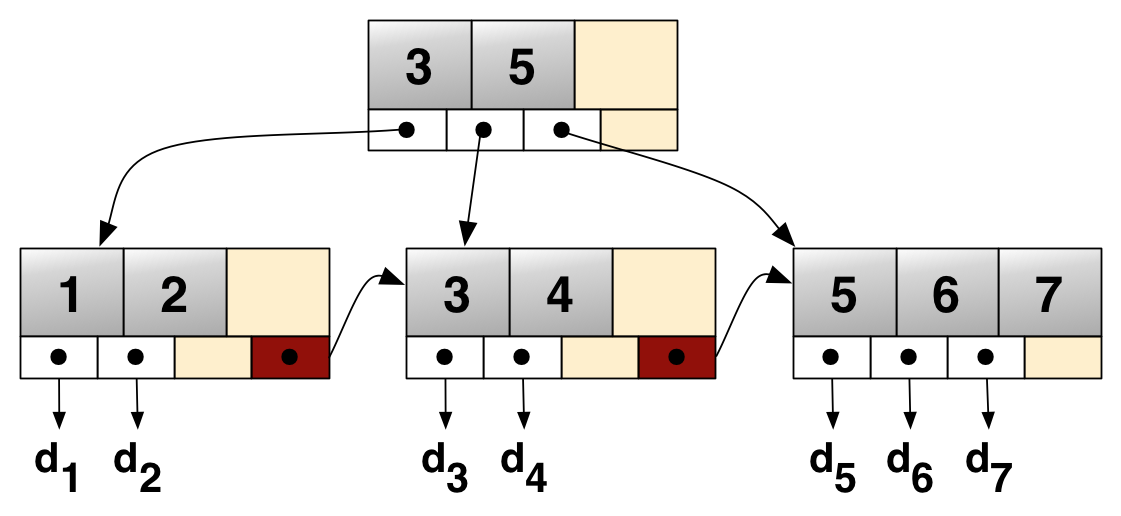
\includegraphics[width=0.8\columnwidth]{image/Bplustree.png}}
    \caption{B+树的基本结构}
    \label{fig: bplustree}
    \end{center}
\end{figure}

在确定了使用的数据结构后,考虑该模块的设计。首先确认的是,我们应该允许用户对商品名称的修改,所以为了能够正常索引,如之前\texttt{MarketingTask}类一样,我们需要为每个商品设计独一无二的ID。在这里考虑和此前相同的“时间戳-UUID”方案。为了和\texttt{MarketingTask}类的ID区分,我们额外为商品类的ID前缀增加了“PROD-”。其次,我们需要确认模块需要支持哪些查找方式。首先针对商品名的查找可以通过Trie树实现。其次需要支持对价格的查询,包括对价格的精确查询和对价格的范围查询。最后,作为商品唯一的不变属性,我们还希望能够直接通过ID查询。为了同时支持这些查询方式,同时让存储最优,我们借用了数据库中主键和次键的概念,定义主键为商品ID,次键为商品价格和商品名称。对于主键,我们采用一个B+树来储存“键-对象”键值对,而对于次键,我们仅存储“商品名-商品ID”和“价格-商品ID”键值对\footnote{注意,由于本模块仅实现原理,并未实现真正的外存操作,所以这样的设计对该模块本身的效率提升不大,但是这种设计思路在真实环境中有许多好处。}。

值得注意的是,完整的B+树实现较为复杂。B+树本身就存在检查叶节点和内部节点的上溢和下溢,并相应分裂、借用邻居键、合并等操作,有大量需要实现的细节。不仅如此,对于完整的B+树,还需要考虑节点与磁盘块的对应(Node-to-Disk-Block Mapping)、节点对象的序列化与反序列化、缓冲池管理、并发控制和恢复等。出于学习目的,以及时间限制,该模块的所有操作均在内存内直接完成,仅仅完整体现了B+树的核心思想和方法。


\subsubsection{功能实现}
\begin{figure}[t]
    \begin{center}
    \centerline{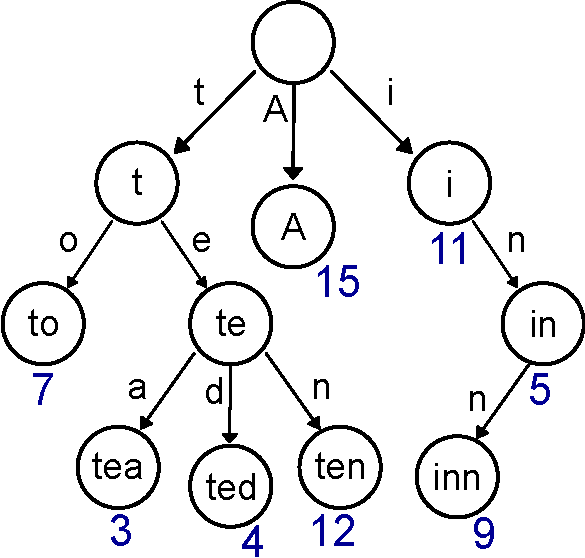
\includegraphics[width=0.4\columnwidth]{image/Trie_example-crop.pdf}}
    \caption{一个保存了8个键的trie结构,"A", "to", "tea", "ted", "ten", "i", "in", "inn"}
    \label{fig: trie example}
    \end{center}
\end{figure}
为了实现上述的功能,在该模块中,总共实现了以下类
\begin{itemize}
    \item \texttt{BPlusTreeNode}
    \item \texttt{BaseBPlusTree}
    \item \texttt{BPlusTreeProducts}
    \item \texttt{BPlusTreeID}
    \item \texttt{TrieNode}
    \item \texttt{ProductPrefixTrie}
    \item \texttt{Product}
    \item \texttt{ProductManager}
\end{itemize}
其中,\texttt{BPlusTreeNode}为B+树的节点类,定义了叶节点和内部节点的不同行为,且为不同的节点提供了键数量上溢和下溢的检查(根节点除外)和是否可以给兄弟节点借用键的检查。\texttt{BaseBPlusTree}是一个B+树的基类,它定义了B+树的一些基本行为,包括节点分裂、节点借用、节点合并、对上溢和下溢的处理等。\texttt{BPlusTreeProducts}和\texttt{BPlusTreeID}继承了这个基类,同时根据不同的存储目的实现了不同的查找、删除、插入逻辑。具体而言,\texttt{BPlusTreeProducts}中每个值包含的是一个列表,列表中存储的是相同价格的商品ID,\texttt{BPlusTreeID}中每个值是一个\texttt{Product}对象,所以他们在具体的插入查找删除逻辑上存在一些差异,且\texttt{BPlusTreeProducts}还额外支持了查找一定价格范围内所有商品ID。

\texttt{TrieNode}定义了Trie树的节点,每个节点代表一个字符,并且额外存在一个布尔变量用来标记该节点是否为一个字段的末尾,如果布尔变量为真,那么该节点存储一个包含所有同名商品的ID的集合。基于这个类,\texttt{ProductPrefixTrie}实现了存储商品名的Trie树,不仅实现了正常插入、前缀匹配逻辑,还实现了一个基于回溯的节点删除逻辑,与标准的Trie树相比,这样优化了存储空间,减少了冗余节点数量。

最后是\texttt{Product}和\texttt{ProductManager}类。与\texttt{MarketingTask}类类似,\texttt{Product}类通过\texttt{@property}和setter来规定对其属性的访问和修改操作。\texttt{ProductManager}基于前一节的分析,实现了通过两个B+树和一个Trie树的高效增删改查和前缀匹配操作。

该模块内容较多,且有大量类似重复逻辑,所以在此选择较为重要的部分讲解,具体实现过程请参考源代码。下面以\texttt{BaseBPlusTree}和\texttt{BPlusTreeID}为例讲解B+树的实现。首先简要介绍\texttt{BPlusTreeNode}

\texttt{BPlusTreeNode}

该类用于表示B+树中的内部节点和叶节点。对于内部节点和叶节点具有以下通用属性
\begin{itemize}
    \item \texttt{order}
    \item \texttt{is\_leaf}
    \item \texttt{parent}
    \item \texttt{keys}
\end{itemize}
分别用来表示B+树的阶(用于计算节点键数的上下界),是否为叶节点,父节点的指针和键列表。对于内部节点,有属性
\begin{itemize}
    \item \texttt{chileren}
\end{itemize}
用于表示子节点的索引,而对于叶子节点有属性
\begin{itemize}
    \item \texttt{values}
    \item \texttt{next\_leaf}
    \item \texttt{prev\_leaf}
\end{itemize}
分别用来存储每个键对应的值,指向左兄弟的指针和指向右兄弟的指针用于快速查找。同时实现了以下方法:
\begin{itemize}
    \item \texttt{is\_overflow()}:检查节点的键数量是否超过上限
    \item  \texttt{min\_keys\_for\_node()}:返回此节点(如果非根)应包含的最小键数
    \item  \texttt{is\_deficient()}:检查节点是否下溢
    \item  \texttt{can\_lend\_key()}:检查节点是否有富余的键可以借给兄弟节点(即键数量 > 最小允许数量)不考虑根节点,因为根节点不参与这种借用
    \item  \texttt{get\_num\_keys()}:返回当前节点中的键数量
    \item  \texttt{get\_num\_children()}:返回当前内部节点的子节点数量
\end{itemize}

下面首先讲解\texttt{BPlusTreeID},将一些细节操作抽象到基类之后的具体增删查操作的实现\footnote{对于B+树的改操作,本质上是查找后删除,然后重新插入新的节点,所以被整合进了\texttt{ProductManager}类}。

\texttt{search()}:精确查找具有指定ID的商品

首先通过辅助函数\texttt{\_find\_leaf\_node()}找到键所在的叶节点,然后在叶节点中遍历查找具体的对象实现查找

\texttt{insert()}:向B+树中插入一个商品

首先通过\texttt{\_find\_leaf\_node()}找到键应该存入的叶节点,然后使用\texttt{\_insert\_into\_leaf()}将值插入该节点,随后检查当前节点是否出现上溢,如果上溢,利用辅助函数\texttt{\_split\_leaf()}实现上溢处理。

\texttt{\_insert\_into\_leaf()}:辅助函数:将商品插入到指定的叶节点中

由于叶节点中键的存放是有序的,所以通过二分查找寻找键应该插入的位置后直接插入

\texttt{delete()}:从B+树中删除一个具有指定product\_id的商品

首先通过\texttt{\_find\_leaf\_node()}找到键应该所在的叶节点,然后检查该节点内是否存在该键,如果存在,则直接从键列表和值列表中均弹出该键值对,最后检查删除该键后节点是否出现下溢。需要注意的是,对于根节点需要额外判断,因为B+树允许根节点为叶节点时不设置下溢阈值.

可以看到,\texttt{BPlusTreeID}的实现较为简单,是因为\texttt{BaseBPlusTree}隐藏了大量的底层细节,下面一一讲解

\texttt{\_find\_leaf\_node()}:根据输入的键,找到这个键对应的叶子结点

从根开始,查找输入键在每一个内部节点应该进入的下一个位置,直到到达叶子结点

\texttt{\_split\_leaf()}:辅助函数:分裂一个已满的叶节点

创建一个新的叶子结点,然后从原节点差不多中间的位置裂开,将右边的键值对赋予新的叶子节点,然后在原节点中删除,随后更新节点之间的链表指针,最后以右边节点的第一个键作为上推到父节点的键,使用\texttt{\_insert\_into\_parent()}上推到父亲节点。

\texttt{\_insert\_into\_parent()}:辅助函数:在父节点中插入一个键和指向新右子节点的指针

获取当前节点的父节点,如果父节点为None,说明当前节点为根节点,对于这种情况,需要创建一个新的以属性为内部节点的根节点,否则,找到在父节点孩子列表中的插入位置,同步更新父节点的键列表和值列表,最后检查父节点是否因为这次插入溢出,如果溢出,使用\texttt{\_split\_internal\_node()}处理。

\texttt{\_split\_internal\_node()}:辅助函数:分裂一个已满的内部节点

类似\texttt{\_split\_leaf()}的实现逻辑,只是需要注意对于内部节点,键只表示左右界,而不像叶节点的一一对应,所以需要注意分裂位置和修改位置的选取。当实现分裂后,重新调用\texttt{\_insert\_into\_parent()}将分裂得到的新键上插到父节点。

\texttt{\_handle\_leaf\_node\_underflow()}:处理叶节点下溢。尝试从兄弟节点借用,否则进行合并

根据当前节点的位置以及左右兄弟是否可以借出键(借出后不会导致下溢),考虑以下四种操作:和左兄弟借用键、和右兄弟借用键、和左兄弟合并、和右兄弟合并。如果发生了合并,需要更新父节点中的键,导致父节点中的键变少,所以检查父节点是否发生下溢,调用\texttt{\_handle\_internal\_node\_underflow()}处理。如果父节点是根节点,也需要调用上述函数,在该函数中处理根节点的各种情况。

\texttt{\_handle\_internal\_node\_underflow()}:处理内部节点下溢。尝试从兄弟节点借用,否则进行合并

同样的借用、合并逻辑,只是需要额外对根节点进行判断,当前节点是根节点且没有键了,那么需要降低树高,将唯一一个孩子节点上提作为新的根节点(如果根节点作为内部节点没有键了,说明它只有一个孩子)。如果不是根节点,同样的,如果发生了合并,需要检查其父节点是否出现下溢,并递归调用该函数。

关于Trie树的实现,较为简单,所以在此不做更多的分析。


\subsubsection{时间和空间复杂度分析}
\begin{table}[t]
    \centering
    \caption{BPlusTreeProducts方法复杂度分析 (N为商品条目总数, m为B+树阶数)}
    \label{tab: bplustree_complexity}
    \begin{tabular}{lll}
    \toprule
    方法& 时间复杂度& 空间复杂度 \\
    \midrule
    \texttt{insert()} & $O^*(m \log_m N)$ & $O(m)$ \\
    \texttt{search\_exact()} & $O^*(\log_m N \cdot \log m)$ & $O(1)$ \\
    \texttt{search\_range()} & $O^*(\log_m N \cdot \log m)$ & $O(1)$ \\
    \texttt{delete()} & $O^*(m \log_m N )$ & $O(m)$ \\
    \bottomrule
    \end{tabular}
\end{table}
本节会对该模块中使用的B+树和Trie树的基本操作进行时间和空间复杂度进行分析,其他操作均为这些操作的叠加,所以不另外做分析。对于B+树,如上节,选取\texttt{BPlusTreeProducts}为例子作为分析,两B+树性质类似,对于另一个B+树不做单独分析。

首先考虑\texttt{BPlusTreeProducts}。设该B+树的order为$m$,存储的商品数量为$N$:

\begin{itemize}
    \item \texttt{insert()}:对于插入,类似二叉搜索树的插入,只是每个节点延伸的子节点数量为$O(m)$,所以单独插入的时间复杂度为$O^*(\log m \cdot \log_m N)$,为每一步的二分查找乘以树高,但是如果发生了节点分裂,就会变成$O^*(m\log_m N)$,所以最终的时间复杂度为$O^*(m\log_m N)$。而空间复杂度考虑分裂节点时创建的新节点,为$O(m)$。
    \item \texttt{search\_exact()}:对于搜索,其主导时间复杂度还是查找叶节点,所以时间复杂度为$O^*(\log m \cdot \log_m N)$,空间复杂度与查找到的节点数量有关,这里假设每次查找返回的商品数量为$O(1)$,即为空间复杂度。
    \item \texttt{search\_range()}:对于范围搜索,时间复杂度依赖其范围有多大,假设范围横跨的节点数量为$O(1)$(范围不太大),那么范围搜索的时间复杂度仍然为$O^*(\log m \cdot \log_m N)$,空间复杂度为$O(1)$\footnote{在真实场景中,可能横跨节点极大,这里只是简化分析,如果横跨节点数量很大,那么需要在时间复杂度中加入这一项,以及相应的添加节点的时间成本。同样的,对于下文的Trie树,对于复杂度严重依赖查找到的数量的操作,我也做了类似的简化。}。
    \item \texttt{delete()}:这一步的主导复杂度为处理下溢,所以时间复杂度为$O^*(m\log_m N)$,空间复杂度为$O(m)$。
\end{itemize}

分析的总结可以参考表\ref{tab: bplustree_complexity}。下面分析\texttt{ProductPrefixTrie}的时间和空间复杂度,设$L$为输入的商品名或前缀长度
\begin{itemize}
    \item \texttt{insert()}:插入每一步对商品的一个字符拓展一个节点,所以时间复杂度为$O(L)$,空间复杂度为$O(L)$
    \item \texttt{get\_product\_ids\_with\_prefix()}:考虑该前缀下的商品数量不太多,所以搜索不会覆盖大部分的Trie树,因此主要复杂度仍然在搜索前缀上,时间和空间复杂度均为$O(L)$。
    \item \texttt{delete()}:搜索和回溯清理的时间和空间复杂度均为$O(L)$,所以总的时间复杂度和空间复杂度为$O(L)$
\end{itemize}

对\texttt{ProductPrefixTrie}分析的总结可以查看表\ref{tab: trie_complexity}。

\section{改进思路}
这一节主要涵盖项目可以改进的算法和系统设计设计方向。由于时间因素,许多在系统成型后的想法无法推倒重来,所以总结如下。下面每一个子章节均考虑的是对于具体任务的提升思路。对于系统整体,一个比较重要的提升方向是,当前系统内的数据结构均不是线程安全的,这意味着直接拿到并发场景下可能会出现错误,导致系统内存储的数据偏离其规则。虽然当前系统已经进行了相当充分的类型检查、数值检查等操作,但是这也只能发现问题,而不能解决问题,且由于没有操作记录,不能回滚操作,所以未来可以让系统适配多线程场景,且需要设置操作记录,以便当出现问题时会滚数据。
\label{sec: improvement}


\subsection{营销任务优先调度模块}
在考虑营销任务前置依赖的优先调度时,该模块目前仅仅考虑在不存在前置依赖的任务中进行优先度排序,从中选择优先度最高的执行。然而,在实际环境中,可能存在某个前置任务虽然不紧急,但是其后置任务十分紧急的情况,而当前的算法无法捕捉这种后继任务的重要性。后续可以考虑的优化方向为,由于任何一个有向无环图可以通过若干条不相交的路径进行路径覆盖,因此考虑将依赖图拆分成多条路径,对于每一条路径进行整体的优先级排序。这一步需要定义路径优先级,目前的想法是可以定义一个衰减因子$\gamma$\footnote{本质是一个惩罚项,越靠后的高优先级任务需要提前完成的代价越大。},则路径中某个节点$o$对路径优先级的影响力可以计算为
\begin{align*}
    IF(o) = \gamma^k \text{priority}(o),
\end{align*}
其中$k$为路径起点到节点$o$的步数,衰减因子可以由任务的时效性决定,时效性越强的任务,$\gamma$越接近于$1$。通过对路径优先级进行排序,来决定优先执行哪一条路径的第一个任务。当有任务被完成时,重新计算路径优先级。该想法由于时间原因,无法在项目中实现,故在此陈述。


\subsection{客户网络与影响力传播分析模块}
对于客户重要性评价任务,本项目只选取了三个指标进行计算。如果要用于真实环境的商业分析,也许可以考虑更多指标,然后对这些指标进行统计分析,综合筛选最为重要的客户。

对于计算客户的影响范围任务,目前采用的方案是定义了一个最小影响力阈值,对路径影响力小余阈值的路径进行剪枝处理。然而在实际环境中,这样的方式存在一个较大的问题:对于不同大小和复杂程度的图,合理的最小影响力阈值是不同的。当前需要指定的阈值在真实场景中可能会严重偏离目标,所以需要自适应调整该阈值的逻辑,或者更换全新的,本身就考虑了图结构的指标来实现面对不同规模和复杂度的图,都能较为准确的反映目标。

最后,当前的算法设计假设了一开始存在一个图,随后对图进行分析,即假设数据是offline的,所以每次图更新都需要重新跑一次算法。然而这样的算力开销在数据量较大的时候会比较大。假设真实系统的数据是在线(online)获取的,当前的分析模块可以通过记录当前的遍历结果,结合新增的影响力关系直接计算新的影响网络下的指标,这样虽然会增加内存开销,但是避免了每次更新都完整遍历一遍整个影响力图,是一个潜在的优化方向。

\begin{table}[t]
    \centering
    \caption{ProductPrefixTrie方法复杂度分析 (L为输入的名称或前缀长度)}
    \label{tab: trie_complexity}
    \begin{tabular}{lll}
    \toprule
    方法& 时间复杂度& 空间复杂度 \\
    \midrule
    \texttt{insert()} & $O(L)$ & $O(L)$ \\
    \texttt{get\_product\_ids\_with\_prefix()()} & $O(L)$ & $O(L)$ \\
    \texttt{delete()} & $O(L)$ & $O(L)$ \\
    \bottomrule
    \end{tabular}
\end{table}

\subsection{商品数据检索模块}

本模块由于其实现难度较大,有需要可以改进的地方。本质上是需要实现一个关系型数据库来对大量数据进行高效的存储。同时,完整的B+树也是一个可以完善的重点,具体需要实现的内容在前文已经讨论过了,所以不再过多赘述。关于前缀匹配,当前的Trie树的实现方案虽然可以通过一些方式实现对外存的读取,在外存中往往会消耗大量时间,这里存在许多可以改进的方向。一个比较简单的思路是将B+树和Trie树结合起来,将Trie树作为B+树的一个值存储起来,这样可以在一次读取中实现对部分Trie树的加载,然后利用Trie树在内存中的高效性实现高效的前缀匹配。关于在外存中进行前缀匹配,也有许多其他的方案,如Generalized Suffix Tree(GST)等。

\section{总结}
本报告详细阐述了为新兴数据驱动商业决策平台设计的底层智能数据管理系统。该系统核心围绕三大模块构建:营销任务优先调度、客户网络与影响力传播分析以及商品数据检索,旨在为上层决策提供坚实的数据支撑。

在设计与实现过程中,针对营销任务优先调度模块,通过结合任务的紧急度与影响力定义优先级,并利用可更新最大堆(UpdatableMaxHeap)和任务依赖有向图(TaskDependencyGraph)实现了高效的任务管理、状态监控(Pending, Ready, Complete)以及考虑前置依赖的任务执行与展示。进一步,报告对该模块所用数据结构及算法的时间和空间复杂度进行了分析。

对于客户网络与影响力传播分析模块,系统基于客户间的加权有向图,采用了加权度中心性(包括WIDC和WODC)与PageRank算法来评估客户的重要性。同时,通过深度优先搜索结合路径影响力阈值,实现了对客户影响范围的分析。此模块同样包含了相关数据结构如CustomerGraph及算法的复杂度分析。

在商品数据检索模块方面,为了应对大量商品数据并实现高效的外存操作,系统采用了B+树作为主要数据结构来管理商品信息(包括ID、价格、热度等),支持高效的增删改查及价格范围搜索。同时,利用Trie树实现了商品名称的前缀搜索功能。这一部分也对B+树和Trie树的操作复杂度进行了分析。

此外,报告还探讨了各模块未来的改进思路。例如,营销任务调度模块可以引入路径优先级的概念,综合考量整个任务链的紧急性;客户影响力分析模块可以探索自适应阈值调整或引入更多维度的客户重要性评价指标,并考虑在线数据更新的算法优化;商品数据检索模块则可以进一步完善B+树的实现,使其更贴近真实外存操作,并探索如GST等更优的前缀匹配方案。

综上所述,本项目成功设计并分析了一个多模块的智能数据管理系统,为商业决策平台提供了关键的数据处理与分析能力。通过对各模块功能、实现及复杂度的详细阐述,以及对未来改进方向的思考,本报告为该系统的进一步开发和优化奠定了基础。


\bibliographystyle{plainnat}
\bibliography{reference}

\newpage
\appendix

\section{系统测试Demo}
\label{sec: demo}
该项目在\texttt{app.py}中提供了一些Demo,用以演示系统的功能,可以在项目根目录下运行
\begin{align*}
    \mathtt{python \; app.py}
\end{align*}
来查看运行结果。运行结果也在此展示。
\begin{tiny}
\begin{verbatim}
    开始演示数据驱动商业决策平台 - 底层数据处理模块...

========== 客户网络分析演示 ==========
客户图构建完毕。

--- 客户重要性 (模拟 PageRank) ---
  David: 0.2711
  Bob: 0.2672
  Eve: 0.2649
  Charlie: 0.1668
  Alice: 0.0300

--- 客户重要性 (加权出度) ---
  Alice: 1.70
  Bob: 1.60
  David: 0.90
  Charlie: 0.50
  Eve: 0.20

--- 客户影响力传播 (模拟,无限制) ---
  客户 'Alice' 能影响到 (阈值 0.1): {'Charlie', 'David', 'Eve', 'Bob'}
  客户 'Bob' 能影响到 (阈值 0.1): {'Charlie', 'David', 'Eve'}

========== 商品目录演示 ==========
商品添加完毕。

--- 按ID查找商品 (P1) ---
  Product(id='PROD-20250515211921800467-a87dbb17282e4a09b2dd9336117e6146', name='智能手机X', price=799.99, heat=95.00)

--- 价格在 [100.00, 300.00] 的商品 ---
  Product(id='PROD-20250515211921800616-22672751af4e48dcb6925db7bb206e16', name='无线耳机Air', price=159.00, heat=90.00)
  Product(id='PROD-20250515211921800604-f2d4445c3aee4119a80bd6c057827ce9', name='智能手表S2', price=249.50, heat=88.00)

--- 价格在 [1000.00, 2000.00] 的商品 ---
  Product(id='PROD-20250515211921800585-867a6ec209c044c7bd482d663e0c83a7', name='笔记本电脑Pro', price=1299.00, heat=92.00)

--- 按前缀 '智能' 推荐 (Top 2 热度) ---
  Product(id='PROD-20250515211921800657-927e3040384040469a3fbb5ca2e3c29c', name='智能手机X Plus', price=999.99, heat=98.00)
  Product(id='PROD-20250515211921800467-a87dbb17282e4a09b2dd9336117e6146', name='智能手机X', price=799.99, heat=95.00)

--- 按前缀 '笔记' 推荐 (Top 1 热度) ---
  Product(id='PROD-20250515211921800585-867a6ec209c044c7bd482d663e0c83a7', name='笔记本电脑Pro', price=1299.00, heat=92.00)

--- 更新商品 'PROD-20250515211921800585-867a6ec209c044c7bd482d663e0c83a7' (笔记本电脑Pro) ---

--- 更新后 ---
  Product(id='PROD-20250515211921800585-867a6ec209c044c7bd482d663e0c83a7', name='笔记本电脑Pro', price=1299.00, heat=92.00)

--- 更新后,价格在 [1300.00, 1500.00] 的商品 ---
  (无结果)

--- 删除商品 'PROD-20250515211921800616-22672751af4e48dcb6925db7bb206e16' (无线耳机Air) ---

--- 删除后查找 (应为None或无结果) ---
  None

--- 删除后,按前缀 '无线' 推荐 ---
  (无结果)

========== 营销任务优先级调度演示 ==========
初始任务添加完毕。

--- 初始Top 3就绪任务 ---
  MarketingTask(id='20250515211921800894-073726c7886e415ababc0f13b520f2c5', name='B:社交媒体预热', urgency=8.00, influence=8.00, priority=64.00, status='READY')
  MarketingTask(id='20250515211921800930-430bcfa745734042aa846aca1d5b7f95', name='E:网红直播推广', urgency=6.00, influence=9.00, priority=54.00, status='READY')
  MarketingTask(id='20250515211921800874-2fd4c57464b9456fa0331d860a5e2314', name='A:新品发布会策划', urgency=5.00, influence=10.00, priority=50.00, status='READY')

--- 添加依赖关系 ---
依赖关系添加完毕。

--- 添加依赖后Top 5就绪任务 ---
  MarketingTask(id='20250515211921800874-2fd4c57464b9456fa0331d860a5e2314', name='A:新品发布会策划', urgency=5.00, influence=10.00, priority=50.00, status='READY')
  MarketingTask(id='20250515211921800920-223d9f2123e54809bcb219e24c84bcb2', name='D:渠道合作洽谈', urgency=7.00, influence=6.00, priority=42.00, status='READY')
  MarketingTask(id='20250515211921800909-108dae6f0abf4f5cbf2d66c0eb2bf13b', name='C:广告素材设计', urgency=3.00, influence=10.00, priority=30.00, status='READY')
  MarketingTask(id='20250515211921800939-ba6ffe181876473baa7aad1b15a26d04', name='F:官网信息更新', urgency=4.00, influence=7.00, priority=28.00, status='READY')

--- 按优先级顺序执行任务 ---

第 1 次执行:
  已执行: A:新品发布会策划 (ID: 20250515211921800874-2fd4c57464b9456fa0331d860a5e2314, Prio: 50.0)

---   当前Top 3就绪任务 ---
  MarketingTask(id='20250515211921800920-223d9f2123e54809bcb219e24c84bcb2', name='D:渠道合作洽谈', urgency=7.00, influence=6.00, priority=42.00, status='READY')
  MarketingTask(id='20250515211921800909-108dae6f0abf4f5cbf2d66c0eb2bf13b', name='C:广告素材设计', urgency=3.00, influence=10.00, priority=30.00, status='READY')
  MarketingTask(id='20250515211921800939-ba6ffe181876473baa7aad1b15a26d04', name='F:官网信息更新', urgency=4.00, influence=7.00, priority=28.00, status='READY')

第 2 次执行:
  已执行: D:渠道合作洽谈 (ID: 20250515211921800920-223d9f2123e54809bcb219e24c84bcb2, Prio: 42.0)

---   当前Top 3就绪任务 ---
  MarketingTask(id='20250515211921800909-108dae6f0abf4f5cbf2d66c0eb2bf13b', name='C:广告素材设计', urgency=3.00, influence=10.00, priority=30.00, status='READY')
  MarketingTask(id='20250515211921800939-ba6ffe181876473baa7aad1b15a26d04', name='F:官网信息更新', urgency=4.00, influence=7.00, priority=28.00, status='READY')

第 3 次执行:
  已执行: C:广告素材设计 (ID: 20250515211921800909-108dae6f0abf4f5cbf2d66c0eb2bf13b, Prio: 30.0)

---   当前Top 3就绪任务 ---
  MarketingTask(id='20250515211921800894-073726c7886e415ababc0f13b520f2c5', name='B:社交媒体预热', urgency=8.00, influence=8.00, priority=64.00, status='READY')
  MarketingTask(id='20250515211921800939-ba6ffe181876473baa7aad1b15a26d04', name='F:官网信息更新', urgency=4.00, influence=7.00, priority=28.00, status='READY')

第 4 次执行:
  已执行: B:社交媒体预热 (ID: 20250515211921800894-073726c7886e415ababc0f13b520f2c5, Prio: 64.0)

---   当前Top 3就绪任务 ---
  MarketingTask(id='20250515211921800930-430bcfa745734042aa846aca1d5b7f95', name='E:网红直播推广', urgency=6.00, influence=9.00, priority=54.00, status='READY')
  MarketingTask(id='20250515211921800939-ba6ffe181876473baa7aad1b15a26d04', name='F:官网信息更新', urgency=4.00, influence=7.00, priority=28.00, status='READY')

第 5 次执行:
  已执行: E:网红直播推广 (ID: 20250515211921800930-430bcfa745734042aa846aca1d5b7f95, Prio: 54.0)

---   当前Top 3就绪任务 ---
  MarketingTask(id='20250515211921800939-ba6ffe181876473baa7aad1b15a26d04', name='F:官网信息更新', urgency=4.00, influence=7.00, priority=28.00, status='READY')

第 6 次执行:
  已执行: F:官网信息更新 (ID: 20250515211921800939-ba6ffe181876473baa7aad1b15a26d04, Prio: 28.0)

---   当前Top 3就绪任务 ---
  (无结果)

--- 所有预期任务执行完毕 ---

--- 所有任务最终状态 ---
  MarketingTask(id='20250515211921800874-2fd4c57464b9456fa0331d860a5e2314', name='A:新品发布会策划', urgency=5.00, influence=10.00, priority=50.00, status='COMPLETED')
  MarketingTask(id='20250515211921800894-073726c7886e415ababc0f13b520f2c5', name='B:社交媒体预热', urgency=8.00, influence=8.00, priority=64.00, status='COMPLETED')
  MarketingTask(id='20250515211921800909-108dae6f0abf4f5cbf2d66c0eb2bf13b', name='C:广告素材设计', urgency=3.00, influence=10.00, priority=30.00, status='COMPLETED')
  MarketingTask(id='20250515211921800920-223d9f2123e54809bcb219e24c84bcb2', name='D:渠道合作洽谈', urgency=7.00, influence=6.00, priority=42.00, status='COMPLETED')
  MarketingTask(id='20250515211921800930-430bcfa745734042aa846aca1d5b7f95', name='E:网红直播推广', urgency=6.00, influence=9.00, priority=54.00, status='COMPLETED')
  MarketingTask(id='20250515211921800939-ba6ffe181876473baa7aad1b15a26d04', name='F:官网信息更新', urgency=4.00, influence=7.00, priority=28.00, status='COMPLETED')

==============================
所有演示场景执行完毕。
\end{verbatim}
\end{tiny}

\section{单元测试代码}
该项目代码通过了本节提供的全部的$150$个单元测试,充分体现了代码的正确性。可以在项目根目录下运行命令
\begin{align*}
    \mathtt{python \; \text{-}m \; unittest}
\end{align*}
来验证单元测试。
\label{sec: unittest}
% 每个部分的测试用例都写成一个subsection,在最开头的地方写明所有的测试用例都通过了
\subsection{营销任务优先调度模块}
这一部分包括营销任务优先调度模块在实现时用到的所有单元测试代码。
\subsubsection{test\_dependency\_graph.py}
\lstinputlisting[caption=$\mathtt{test\_dfs\_influence.py}$]{../tests/test_dependency_graph.py}

\subsubsection{test\_updatable\_max\_heap.py}
\lstinputlisting[caption=$\mathtt{test\_dfs\_influence.py}$]{../tests/test_updatable_max_heap.py}

\subsubsection{test\_marketing.py}
\lstinputlisting[caption=$\mathtt{test\_dfs\_influence.py}$]{../tests/test_marketing.py}

\subsection{客户网络与影响力传播分析模块}
这一部分包括客户网络与影响力传播分析模块在实现时用到的所有单元测试代码。

\subsubsection{test\_customer\_graph.py}
\lstinputlisting[caption=$\mathtt{test\_dfs\_influence.py}$]{../tests/test_customer_graph.py}

\subsubsection{test\_dfs\_influence.py}
\lstinputlisting[caption=$\mathtt{test\_dfs\_influence.py}$]{../tests/test_dfs_influence.py}

\subsubsection{test\_pagerank.py}
\lstinputlisting[caption=$\mathtt{test\_dfs\_influence.py}$]{../tests/test_pagerank.py}

\subsubsection{test\_weighted\_degree\_centrality.py}
\lstinputlisting[caption=$\mathtt{test\_dfs\_influence.py}$]{../tests/test_weighted_degree_centrality.py}

\subsection{商品数据检索模块}
\subsubsection{test\_b\_plus\_tree.py}
\lstinputlisting[caption=$\mathtt{test\_b\_plus\_tree.py}$]{../tests/test_b_plus_tree.py}

\subsubsection{test\_trie.py}
\lstinputlisting[caption=$\mathtt{test\_trie.py}$]{../tests/test_trie.py}

\subsubsection{test\_product.py}
\lstinputlisting[caption=$\mathtt{test\_product.py}$]{../tests/test_product.py}

\section{LLM工具使用说明}
\label{sec: llm}
本项目主要使用Gemini 2.5 pro (preview)和ChatGPT 4o辅助构建。其中,Gemini 2.5 pro (preview)用于验证规划和设计是否合理,以及根据设计目标生成所有的单元测试代码\footnote{已经验证过正确性。},ChatGPT 4o用于关于Python语法等问题,以及项目报告在撰写的过程中\LaTeX 编译相关问题。此外,在B+树的构建中,Gemini 2.5 pro (preview)在帮忙寻找BUG的过程中起到了帮助。此外,\texttt{app.py}中的演示代码也主要由Gemini 2.5 pro (preview)生成。



\end{document}